%! \usetikzlibrary{decorations.pathreplacing,decorations.pathmorphing}
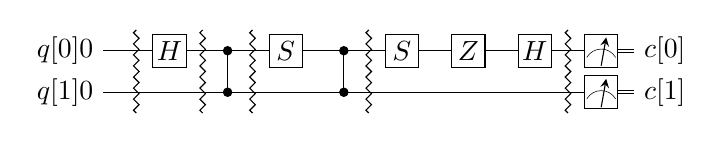
\begin{tikzpicture}[scale=1.000000,x=1pt,y=1pt]
\filldraw[color=white] (0.000000, -7.500000) rectangle (192.000000, 22.500000);
% Drawing wires
% Line 1: q0 W q[0]\ket{0} c[0]
\draw[color=black] (0.000000,15.000000) -- (180.000000,15.000000);
\draw[color=black] (180.000000,14.500000) -- (192.000000,14.500000);
\draw[color=black] (180.000000,15.500000) -- (192.000000,15.500000);
\draw[color=black] (0.000000,15.000000) node[left] {$q[0]\ket{0}$};
% Line 2: q1 W q[1]\ket{0} c[1]
\draw[color=black] (0.000000,0.000000) -- (180.000000,0.000000);
\draw[color=black] (180.000000,-0.500000) -- (192.000000,-0.500000);
\draw[color=black] (180.000000,0.500000) -- (192.000000,0.500000);
\draw[color=black] (0.000000,0.000000) node[left] {$q[1]\ket{0}$};
% Done with wires; drawing gates
% Line 3: BARRIER
\draw[decorate,decoration={zigzag,amplitude=1pt,segment length=4}] (12.000000,-7.500000) -- (12.000000,22.500000);
% Line 4: q0 H
\begin{scope}
\draw[fill=white] (24.000000, 15.000000) +(-45.000000:8.485281pt and 8.485281pt) -- +(45.000000:8.485281pt and 8.485281pt) -- +(135.000000:8.485281pt and 8.485281pt) -- +(225.000000:8.485281pt and 8.485281pt) -- cycle;
\clip (24.000000, 15.000000) +(-45.000000:8.485281pt and 8.485281pt) -- +(45.000000:8.485281pt and 8.485281pt) -- +(135.000000:8.485281pt and 8.485281pt) -- +(225.000000:8.485281pt and 8.485281pt) -- cycle;
\draw (24.000000, 15.000000) node {$H$};
\end{scope}
% Line 5: BARRIER
\draw[decorate,decoration={zigzag,amplitude=1pt,segment length=4}] (36.000000,-7.500000) -- (36.000000,22.500000);
% Line 6: q0 q1
\draw (45.000000,15.000000) -- (45.000000,0.000000);
\filldraw (45.000000, 15.000000) circle(1.500000pt);
\filldraw (45.000000, 0.000000) circle(1.500000pt);
% Line 7: BARRIER
\draw[decorate,decoration={zigzag,amplitude=1pt,segment length=4}] (54.000000,-7.500000) -- (54.000000,22.500000);
% Line 8: q0 G $S$
\begin{scope}
\draw[fill=white] (66.000000, 15.000000) +(-45.000000:8.485281pt and 8.485281pt) -- +(45.000000:8.485281pt and 8.485281pt) -- +(135.000000:8.485281pt and 8.485281pt) -- +(225.000000:8.485281pt and 8.485281pt) -- cycle;
\clip (66.000000, 15.000000) +(-45.000000:8.485281pt and 8.485281pt) -- +(45.000000:8.485281pt and 8.485281pt) -- +(135.000000:8.485281pt and 8.485281pt) -- +(225.000000:8.485281pt and 8.485281pt) -- cycle;
\draw (66.000000, 15.000000) node {$S$};
\end{scope}
% Line 9: q0 q1
\draw (87.000000,15.000000) -- (87.000000,0.000000);
\filldraw (87.000000, 15.000000) circle(1.500000pt);
\filldraw (87.000000, 0.000000) circle(1.500000pt);
% Line 10: BARRIER
\draw[decorate,decoration={zigzag,amplitude=1pt,segment length=4}] (96.000000,-7.500000) -- (96.000000,22.500000);
% Line 11: q0 G $S$
\begin{scope}
\draw[fill=white] (108.000000, 15.000000) +(-45.000000:8.485281pt and 8.485281pt) -- +(45.000000:8.485281pt and 8.485281pt) -- +(135.000000:8.485281pt and 8.485281pt) -- +(225.000000:8.485281pt and 8.485281pt) -- cycle;
\clip (108.000000, 15.000000) +(-45.000000:8.485281pt and 8.485281pt) -- +(45.000000:8.485281pt and 8.485281pt) -- +(135.000000:8.485281pt and 8.485281pt) -- +(225.000000:8.485281pt and 8.485281pt) -- cycle;
\draw (108.000000, 15.000000) node {$S$};
\end{scope}
% Line 12: q0 Z
\begin{scope}
\draw[fill=white] (132.000000, 15.000000) +(-45.000000:8.485281pt and 8.485281pt) -- +(45.000000:8.485281pt and 8.485281pt) -- +(135.000000:8.485281pt and 8.485281pt) -- +(225.000000:8.485281pt and 8.485281pt) -- cycle;
\clip (132.000000, 15.000000) +(-45.000000:8.485281pt and 8.485281pt) -- +(45.000000:8.485281pt and 8.485281pt) -- +(135.000000:8.485281pt and 8.485281pt) -- +(225.000000:8.485281pt and 8.485281pt) -- cycle;
\draw (132.000000, 15.000000) node {$Z$};
\end{scope}
% Line 13: q0 H
\begin{scope}
\draw[fill=white] (156.000000, 15.000000) +(-45.000000:8.485281pt and 8.485281pt) -- +(45.000000:8.485281pt and 8.485281pt) -- +(135.000000:8.485281pt and 8.485281pt) -- +(225.000000:8.485281pt and 8.485281pt) -- cycle;
\clip (156.000000, 15.000000) +(-45.000000:8.485281pt and 8.485281pt) -- +(45.000000:8.485281pt and 8.485281pt) -- +(135.000000:8.485281pt and 8.485281pt) -- +(225.000000:8.485281pt and 8.485281pt) -- cycle;
\draw (156.000000, 15.000000) node {$H$};
\end{scope}
% Line 14: BARRIER
\draw[decorate,decoration={zigzag,amplitude=1pt,segment length=4}] (168.000000,-7.500000) -- (168.000000,22.500000);
% Line 15: q0 M
\draw[fill=white] (174.000000, 9.000000) rectangle (186.000000, 21.000000);
\draw[very thin] (180.000000, 15.600000) arc (90:150:6.000000pt);
\draw[very thin] (180.000000, 15.600000) arc (90:30:6.000000pt);
\draw[->,>=stealth] (180.000000, 9.600000) -- +(80:10.392305pt);
% Line 16: q1 M
\draw[fill=white] (174.000000, -6.000000) rectangle (186.000000, 6.000000);
\draw[very thin] (180.000000, 0.600000) arc (90:150:6.000000pt);
\draw[very thin] (180.000000, 0.600000) arc (90:30:6.000000pt);
\draw[->,>=stealth] (180.000000, -5.400000) -- +(80:10.392305pt);
% Done with gates; drawing ending labels
\draw[color=black] (192.000000,15.000000) node[right] {$c[0]$};
\draw[color=black] (192.000000,0.000000) node[right] {$c[1]$};
% Done with ending labels; drawing cut lines and comments
% Done with comments
\end{tikzpicture}
